\chapter{SYSTEM DESCRIPTION}
       \section{Introduction}
The problem of evaluating the error rate performance of digital
coherently detected systems in the presence of AWGN and carrier
phase error (usually called partially coherent detection) is being
well known and extensively studied in the literature
\cite{schwartz:1966}-[8]. Due to their bandwidth efficiency and
good error rate performance, BPSK and QPSK are the most
investigated systems. In the early studies \cite{schwartz:1966},
\cite{viterbi:1966}, and \cite{lindsey:1973}, the BEP of partially
coherent PSK systems was obtained by numerically integrating the
conditional BEP expression for a fixed phase error over the phase
error statistic. Later on, many authors
\cite{prabhu:mar76},\cite{najib:98},\cite{kaplan:90},\cite{kam:93}
and \cite{some:95} have approached this problem by either deriving
upper and lower bounds (e.g. Chernoff and Jensen bounds) or by
using infinite series approximations (e.g. Fourier and Maclaurin
series) to evaluate the average BEP of such systems.\\

The aforementioned studies did not take channel fading into
account.

\begin{table}[htbp]

  \centering

  \caption{Base Class 1 System Frequecies}

\begin{tabular}{|c|c|c|}

\hline

Band&Reverse Link (MHz)&Forward Link (MHz)\\

\hline

A&1850-1865&1930-1945 \\

\hline

D&1865-1870&1945-1950 \\

\hline

B&1870-1885&1950-1965 \\

\hline

E&1885-1890&1965-1970 \\

\hline

F&1890-1895&1970-1975 \\

\hline

F&1895-1910&1975-1990 \\

\hline

\end{tabular}

  \label{tableintro:2}

\end{table}

And such extension is first targeted by \cite{weber:76}, but
provided only limited detailed results on that. Most recently, the
authors in \cite{simon:mar01} used Maclaurin series to obtain
accurate approximation for the average BEP of partially coherent
BPSK and QPSK for several channel fading models, but large
tracking-loop SNR was assumed in their analysis. For analytical
purposes, it is desirable to have a good approximation, or a tight
bound with less restrict
assumptions on the system.\\

In next section, such lower bound on the error rate performance of
partially coherent BPSK and QPSK Nakagami-m fading systems using
the Jensen's inequality is obtained. In this letter, we basically
extend the work done by Najib and Prabhu [5] by considering
channel fading impairment in the analysis. Section 3 presents
some numerical results while our conclusion is in section 4.\\
\section{ Bounds Derivation}
In this section we will use the Jensen's inequality as in
\cite{najib:98} to derive lower bounds on the error probabilities
of BPSK and QPSK Nakagami-$m$ faded systems under imperfect
carrier phase recovery condition.

\subsection{BPSK Case}
The BEP of BPSK in the presence of AWGN and for a given channel
fading magnitude  and carrier phase error   can be written as
\cite{prabhu:mar76}
\begin{equation}
\label{upper:1}
P_2(e|\alpha,\epsilon)=\frac{1}{2}~\mbox{erfc}\left(\sqrt\gamma_b~
\alpha~\cos\epsilon\right),
\end{equation}
where $E_b/N_0$ is the average signal-to-noise (SNR) per bit.
$\alpha$ is the magnitude of the channel fading gain. Here, we
assumed a slowly Nakagami-$m$ faded channel, hence, $\alpha$ (as
well as $\epsilon$ ) would remain constant over the data symbol
duration $T$ with probability density function (pdf) given as
\begin{equation}
\label{upper:2}
p~(\alpha)=\frac{2m^m}{\Omega^m\Gamma(m)}~\alpha^{2m-1}e^{-\frac{m}{\Omega}~\alpha^2},
\quad \alpha \ge 0
\end{equation}
where $\Omega=E[\alpha^2]$  is the envelope average power,
$\Gamma(.)$ in the Gamma function, and $m\ge0.5$ is the fading
severity parameter. The Nakagami-$m$ distribution spans many
fading distributions. For $m=0.5$  it becomes one-sided Gaussian
distribution, for $m=1$ it becomes Rayleigh distribution, and no
fading case is obtained when $m\rightarrow\infty$.\\

The phase reference error $\epsilon$  is typically modeled by
Tikhonov distribution that given by \cite{viterbi:1966}
\begin{equation}
\label{upper:3} p~(\epsilon)=\frac{e^{\rho_{c}\cos\epsilon}}{2\pi
I_{0}(\rho_c)}, \quad |\epsilon| \le 0
\end{equation}
this distribution is applied when the carrier phase is derived
from unmodulated carrier tone using a first-order phase-locked
loop, as well as, a second order PLL when the SNR in the loop
bandwidth $\rho_c$  is large \cite{viterbi:1966}. In most
practical interest, $\rho_c>>1$ , in which case the rms phase
error $\sigma_\epsilon\simeq\rho_c^{-1/2}$ . However, exact
relationship between $\sigma_\epsilon$ and $\rho_c$ is given in
\cite{viterbi:1966} . $I_n(.)$is the $n$th  order modified Bessel
function of the first kind.\\

The Jensen's inequality states that for any real-valued convex
function $\xi(x)$  in a finite-mean random variable $x$  , the
mean of  $\xi(x)$ is lower bounded by the function value at the
mean of $x$ \cite{viterbi:1966} . Mathematically,
\begin{equation}
\label{upper:4} E\left[\xi(x)\right] \ge\xi \left(E[x]\right),
\end{equation}
where $E[.]$  is the mathematical expectation. Since the error
function in (\ref{upper:1}) is not a convex function in  over the
entire domain of $\epsilon$ , the Jensen inequality is not
applicable to it. Instead by using the simple inequality $\cos x
\le|\cos x|$ , a lower bound of (\ref{upper:1}) can be written as
\begin{equation}
\label{upper:5}
P_2(e|\alpha,\epsilon)\ge\frac{1}{2}~\mbox{erfc}\left(\sqrt{\gamma_b~
\cos^2{\epsilon}}~\alpha\right),
\end{equation}
It can be readily shown that the right hand side of
(\ref{upper:5}) is now a convex function in $\cos^2\epsilon$  for
all $|\epsilon|\le\pi$. By applying Jensen's inequality to
(\ref{upper:5}) the BEP of BPSK under given is lower bounded by
\begin{equation}
\label{upper:6}
P_2(e|\alpha)=E\left[P_2(e|\alpha,\epsilon)\right]|_\epsilon \ge
\frac{1}{2}~\mbox{erfc}\left(\sqrt{\gamma_b~L_2}~\alpha\right),
\end{equation}
where $L_2= E[\cos^2\epsilon]$  is the average power loss in the
BPSK signal due to $\epsilon$ . For the distribution given in
(\ref{upper:3}), one can write
\begin{equation}
\label{upper:7} L_2=\frac{1}{2\pi
I_{0}(\rho_c)}\int\limits_{-\pi}^{\pi}~e^{\rho_c \cos x} \cos
^2x~dx =\frac{1}{2}\left[1+\frac{I_2(\rho_c)}{I_0(\rho_c)}\right].
\end{equation}\\

To eliminate the dependence of (\ref{upper:6}) on $\alpha$ we have
to average it over all values of $\alpha$ . That is
\begin{equation}
\label{upper:8} P_2(e)\ge~\frac{1}{2}
\int\limits_{0}^{\infty}~\mbox{erfc}\left(\sqrt{\gamma_b~L_2}~\alpha\right)p~(\alpha)~d\alpha.
\end{equation}
For the distribution given in (\ref{upper:2}), a closed form
solution of (\ref{upper:8}) can be written using \cite[eq.
6.286.1]{gradeshteyn:1994} as
\begin{equation}
\label{upper:9}
P_2(e)\ge~\frac{m^{m-1}\Gamma(m+1/2)}{2\Omega^m\sqrt\pi~\Gamma(m)\left(\gamma_bL_2\right)^m}~
F\left(m,m+1/2;m+1;-\frac{m}{\Omega\gamma_bL_2}\right),
\end{equation}
where $F(a,b;c;x)$  is the Gaussian hypergeometric function.
% The caption for this figure is too long to appear on a single line in the front matter.  Since it will take more than one line to display in the front matter, single spacing should be used for the caption in the front matter.  To make this happen, you create two versions of the caption: the first includes formatting commands for the front matter, the second is the normal caption that will be displayed with the figure.
% If the caption can appear on a single line in the front matter, just use \caption{caption text goes here}
% added by Darin Brezeale, Fri Jan 11 10:36:42 CST 2008
\begin{figure}[tbp]
\centerline{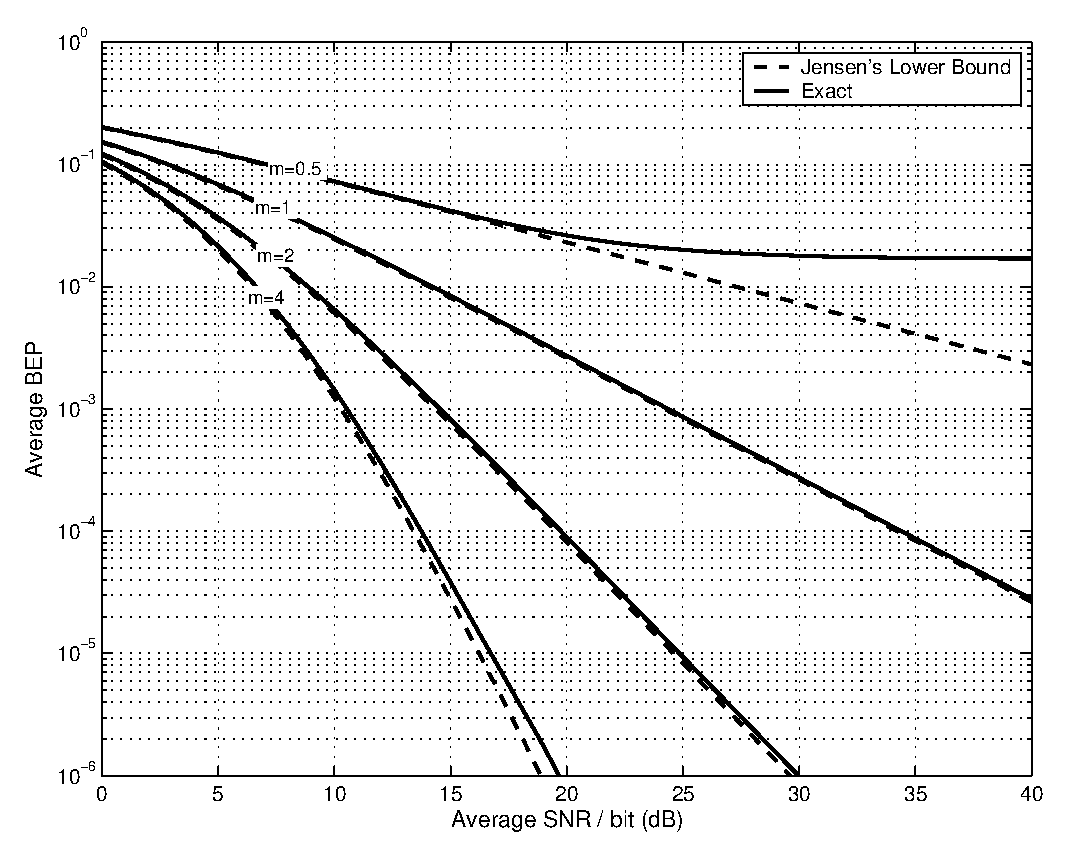
\includegraphics[width=4in]{./upper001.eps}} 
\caption[\vspace{-2ex}{Average bit error probability of partially coherent Nakagami-$m$ \newline \hspace*{0pt} BPSK channel, $\sigma_\epsilon=16^o$}]
{Average bit error probability of partially coherent Nakagami-$m$ BPSK channel, $\sigma_\epsilon=16^o$}
\end{figure}
\subsection{QPSK Case}
The derivation of BEP in the QPSK case will be based on the
assumption that the pair of information bits is mapped into the
four phases using the Gray-encoding scheme in which the adjacent
assigned bits differ only in one position. According to that, the
BEP conditioned on $\alpha$ and $\epsilon$  and assuming equally
probable symbols can be shown to be \cite{prabhu:mar76}
\begin{equation}
\label{upper:10}
P_2(e|\alpha,\epsilon)=\frac{1}{4}~\mbox{erfc}\left(\sqrt{2\gamma_b}~
\alpha~\cos(\epsilon+\pi/4)\right)+\frac{1}{4}~\mbox{erfc}\left(\sqrt{2\gamma_b}~
\alpha~\cos(\epsilon-\pi/4)\right),
\end{equation}
using $2\cos^2(x\mp\pi/4)=1\pm \sin  2x$  , the right hand side of
(\ref{upper:10}) can be bounded by
\begin{equation}
\label{upper:11}
\begin{split}
P_2(e|\alpha,\epsilon)\ge~\frac{1}{4}~\mbox{erfc}\left(\sqrt{\gamma_b(1+\sin2\epsilon)}~
\alpha\right)+\frac{1}{4}~\mbox{erfc}\left(\sqrt{\gamma_b(1-\sin2\epsilon)}~
\alpha\right)\\=\frac{1}{4}~\mbox{erfc}
\left(\sqrt{\gamma_b(1+|\sin2\epsilon|)}~
\alpha\right)+\frac{1}{4}~\mbox{erfc}
\left(\sqrt{\gamma_b(1-|\sin2\epsilon|)}~ \alpha\right).
\end{split}
\end{equation}\\
% The caption for this figure is too long to appear on a single line in the front matter.  Since it will take more than one line to display in the front matter, single spacing should be used for the caption in the front matter.  To make this happen, you create two versions of the caption: the first includes formatting commands for the front matter, the second is the normal caption that will be displayed with the figure.
% If the caption can appear on a single line in the front matter, just use \caption{caption text goes here}
% added by Darin Brezeale, Fri Jan 11 10:36:42 CST 2008
\begin{figure}[tbp]
\centerline{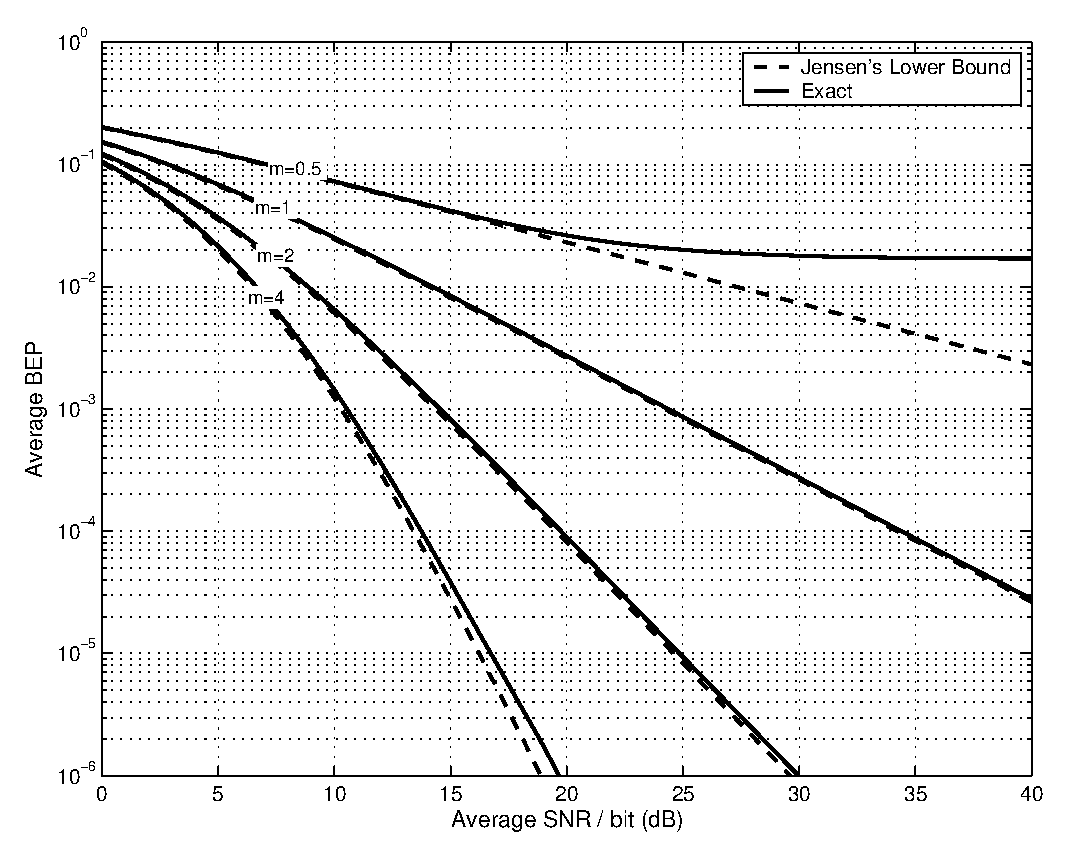
\includegraphics[width=4in]{./upper001.eps}} 
\caption[\vspace{-2ex}{Average bit error probability of partially coherent Nakagami-$m$ \newline \hspace*{0pt} BPSK channel, $\sigma_\epsilon=12^o$}]
{Average bit error probability of partially coherent Nakagami-$m$ BPSK channel, $\sigma_\epsilon=12^o$}
\end{figure}
 Noting that $P_4(e|\alpha,\epsilon)$is a convex function in $|\sin2\epsilon|$ . So, the
average of $P_4(e|\alpha,\epsilon)$ over $\epsilon$ in the last
equation can be further bounded by
\begin{equation}
\label{upper:12} P_2(e|\alpha)\ge ~\frac{1}{4}~\mbox{erfc} \left(
\sqrt{\gamma_b~L_4^+}~ \alpha\right)+\frac{1}{4}~\mbox{erfc}
\left( \sqrt{\gamma_b~L_4^-}~ \alpha \right),
\end{equation}
where $L_4^+=E\left[1+|\sin2\epsilon|\right]$  and
$L_4^-=E\left[1-|\sin2\epsilon|\right]$ are the average power
losses in the QPSK quadrature carriers. Again for Tikhonov phase
error distribution $\epsilon$ , it was shown that \cite{najib:98}
\begin{equation}
\label{upper:13} L_4^+=2-L_4^-=1+\frac{4}{\pi\rho_c^2
I_0(\rho_c)}\left[\rho_c \sinh\rho_c-\cosh\rho_c+1\right].
\end{equation}
Finally, by integrating (\ref{upper:12}) over the pdf of $\alpha$,
the average BEP of QPSK system under investigation is lower
bounded by
\begin{equation}
\label{upper:14}
P_2(e)\ge~\frac{m^{m-1}\Gamma(m+1/2)}{4\Omega^m\sqrt\pi~\Gamma(m)}\left[\vartheta(m,\gamma_b,L_4^+)
+\vartheta(m,\gamma_b,L_4^-)\right],
\end{equation}
where
\begin{equation}
\label{upper:15}
\vartheta(a,b,c)=\frac{F\left(a,a+1/2;a+1;-\frac{a}{\Omega
bc}\right)}{(bc)^a}.
\end{equation}

To summarize, a lower bound for the average BEP of partially
coherent Nakagami-$m$ faded BPSK system is given in
(\ref{upper:9}) and (\ref{upper:7}) and for QPSK system in
(\ref{upper:14}) together with (\ref{upper:13}) and
(\ref{upper:15}). The question is how to evaluate the Gaussian
hypergeometric function $F(m,m+1/2;m+1;x)$that appears in the
bounds expressions. This is what we will investigate in the next
paragraphs.
% The caption for this figure is too long to appear on a single line in the front matter.  Since it will take more than one line to display in the front matter, single spacing should be used for the caption in the front matter.  To make this happen, you create two versions of the caption: the first includes formatting commands for the front matter, the second is the normal caption that will be displayed with the figure.
% If the caption can appear on a single line in the front matter, just use \caption{caption text goes here}
% added by Darin Brezeale, Fri Jan 11 10:36:42 CST 2008
\begin{figure}[tbp]
\centerline{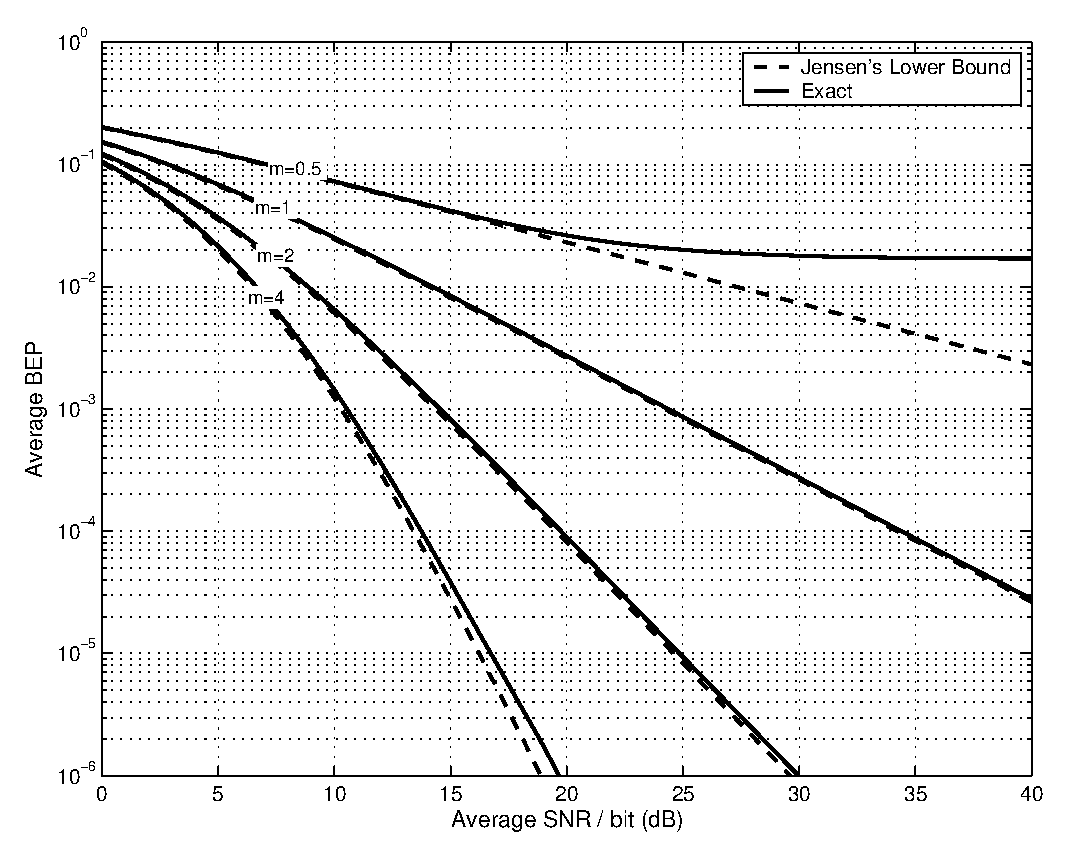
\includegraphics[width=4in]{./upper001.eps}} 
\caption[\vspace{-2ex}{Average bit error probability of partially coherent Nakagami-$m$ \newline \hspace*{0pt} QPSK channel, $\sigma_\epsilon=10^o$}]
{Average bit error probability of partially coherent Nakagami-$m$ QPSK channel, $\sigma_\epsilon=10^o$}
\end{figure}
\subsection{Special Cases}
\subsubsection{For one-sided Gaussian fading ($m$=1/2)}
For $m$=1/2 and by using \cite [eq. 15.1.5]{abramowitz:1972}
\begin{equation}
\label{upper:16} F(1/2,1;3/2;-x^2)=x^{-1}\tan ^{-1}x.
\end{equation}
\subsubsection{For integer $m$}
If m is integer, a recursive down formula\cite [eq.
15.2.12]{abramowitz:1972} can be used to evaluate
$F(m,m+1/2;m+1;x)$  as
\begin{equation}
\label{upper:17}
F(a,b;v-1;x)=c_1(a,b,v,x)F(a,b;v;x)+c_2(a,b,v,x)F(a,b;v+1;x),
\end{equation}
where
\begin{equation}
\label{upper:18}
\begin{split}
c_1(a,b,v,x)=\frac{v[v-1-(2v-a-b-1)x]}{v(v-1)(1-x)}\\
c_2(a,b,v,x)=\frac{(v-a)(v-b)x}{v(v-1)(1-x)}.
\end{split}
\end{equation}
% The caption for this figure is too long to appear on a single line in the front matter.  Since it will take more than one line to display in the front matter, single spacing should be used for the caption in the front matter.  To make this happen, you create two versions of the caption: the first includes formatting commands for the front matter, the second is the normal caption that will be displayed with the figure.
% If the caption can appear on a single line in the front matter, just use \caption{caption text goes here}
% added by Darin Brezeale, Fri Jan 11 10:36:42 CST 2008
\begin{figure}[tbp]
\centerline{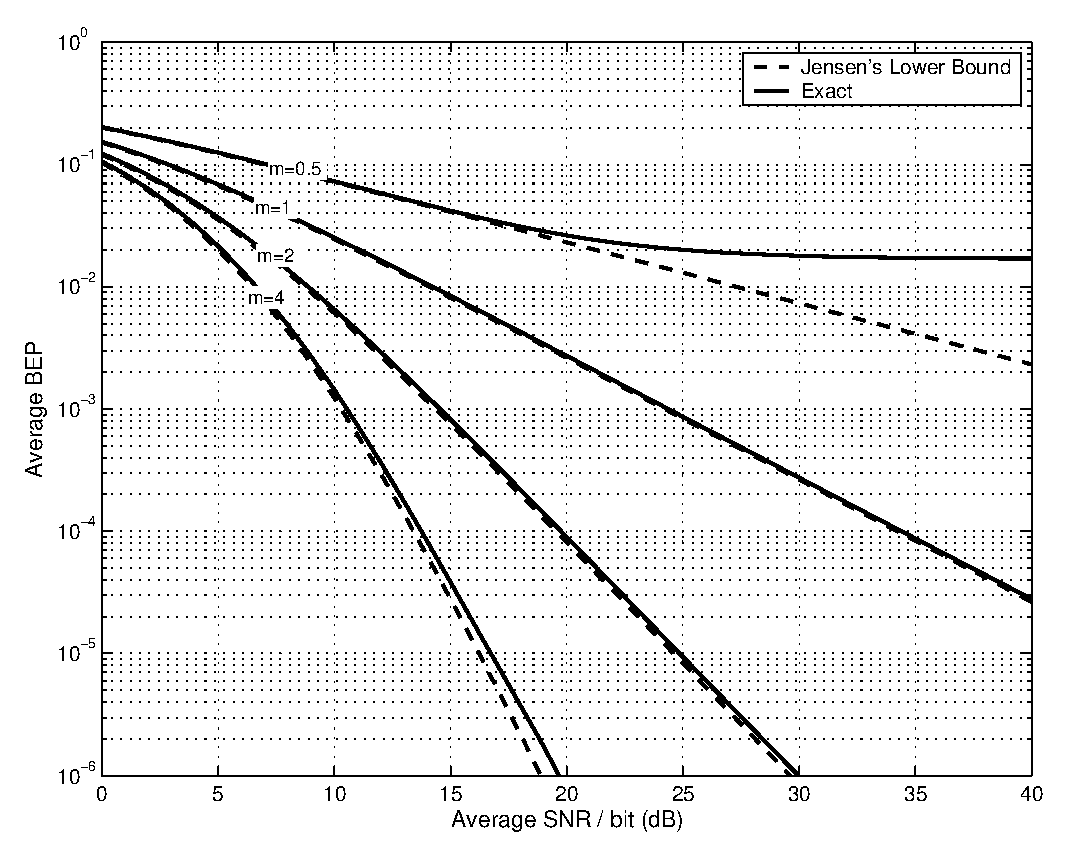
\includegraphics[width=4in]{./upper001.eps}} 
\caption[\vspace{-2ex}{Average bit error probability of partially coherent Nakagami-$m$ \newline \hspace*{0pt} QPSK channel, $\sigma_\epsilon=6^o$}]
{Average bit error probability of partially coherent Nakagami-$m$ QPSK channel, $\sigma_\epsilon=6^o$}
\end{figure}
Let $a=m, b=m+1/2$  , and $v=2m$  and keep calculating till
$v=m+2$ .The seed values to start with can be calculated from
\cite [eq's. 15.1.13,14]{abramowitz:1972} as
\begin{equation}
\label{upper:19}
\begin{split}
F(m,m+0.5;2m+1;x)=2^{2m}\left[1+(1-x)^{1/2}\right]^{-2m}\\
F(m,m+0.5;2m;x)=2^{2m-1}(1-x)^{-1/2}\left[1+(1-x)^{1/2}\right]^{1-2m}.
\end{split}
\end{equation}
Note that for the Rayleigh fading case where $m$=1,
$F(m,m+1/2;m+1;x)$  can be evaluated directly from
(\ref{upper:19}).That is,
\begin{equation}
\label{upper:20}
F(1,3/2;2;x)=2(1-x)^{-1/2}\left[1+(1-x)^{1/2}\right]^{-1}.
\end{equation}

\section{Results}
The bound for BPSK system as given in (\ref{upper:9}) is plotted
in Fig. 1 for different fading parameter $m$ as a function of SNR
at rms phase error of $\sigma_\epsilon=16^o$ and in Fig. 2 at
$\sigma_\epsilon=12^o$ . Similar results for the QPSK case using
(\ref{upper:14}) and (\ref{upper:15}) are presented in Fig. 3 at
$\sigma_\epsilon=10^o$ and in Fig. 4 at $\sigma_\epsilon=6^o$ .
Exact results using Fourier series approximation as derived in
\cite{smadi:TBParticle01} are also shown for validation
purposes.\\

From these figures one can note that the tightness of these bounds
increases as the tracking loop SNR increases (i.e. the rms phase
error $\sigma_\epsilon$  decreases). In the BPSK case, the bound
leads to the exact result at $\sigma_\epsilon\le 12^o$  , while
the bound reaches to the exact results at  $\sigma_\epsilon\le
5^o$ in the QPSK case. We expect that since the QPSK requires much
higher degrees of phase precision than the BPSK case. This is due
to the cross-talk interference between the QPSK quadrature
carriers that introduced by the carrier phase error. Even for
higher rms phase error, the degradation in the error performance
between the derived bounds and the exact results is about 0.3 dB
in the BPSK case at a BEP of $10^{-4}$ and $m$=4, and about 1 dB
in the QPSK case at a BEP of  $10^{-4}$ and $m$=2. These values
corresponding to $\sigma_\epsilon=16^o$ in BPSK case and $\sigma_\epsilon=10^o$ in QPSK case.\\

Also, the figures clearly show that the tightness of the bounds is
better for deeply faded environment (i.e. small $m$) than for less
sever fading environment. This can be explained as follow. The
bounds were derived for the phase error loss terms (
$\cos\epsilon$ in the BPSK case and $1\pm sin2\epsilon$  in the
QPSK case), while exact analysis of the fading effect was done.
That means in deeply fading environment where the system
performance is dominated by fading rather than the phase error,
the bounds will be much tightness. Anyway, for most practical
cases, the bounds remain tight enough to be useful as a design
tool.
\section{Conclusions}
Lower bounds on the error probability of Nakagami-$m$ faded BPSK
and QPSK channels operating in a noisy carrier synchronization
environment have been derived. The derivation is based on the
Jensen's inequality of defined convex functions. These bounds were
shown to be tight for practical range of the rms phase errors.
that, and equally important, is the simplicity of the solution
approach afforded by those bounds compared to the series approach
solution given in \cite{smadi:TBParticle01}, or
\cite{simon:mar01}.
